\documentclass[14pt]{extarticle}
\usepackage{fontspec}
\usepackage{graphicx}
\usepackage{microtype}
\usepackage[
    colorlinks=true,
    linkcolor=blue,
    urlcolor=blue,
    citecolor=blue
]{hyperref}
\setmainfont{Times New Roman}
\setlength{\parindent}{0pt} %to fix next para starting with space!
\setlength{\parskip}{1em} %so next para will have space above!

\title{
     \huge Seminar Report \par
     \Huge M.A.U.I
}
\author{
    Allen Bose
}

\begin{document}
% front page
\maketitle
\pagenumbering{gobble}

% page 1
\newpage
\tableofcontents
\newpage
\pagenumbering{arabic}
\section{
  Cross Platform Applications
 }
\parbox{\linewidth}{
    \setlength{\parskip}{1em}

    A single codebase for multiple platforms.That is the idea behind cross platform applications.Usually when a company makes a software intended for a wider user range they need to make an android app, a web app and a desktop app just to get started.This is quite cumbersome since now you have multiple codebases of varying programming languages that needs to be maintained.
}

\parbox{\linewidth}{
    \setlength{\parskip}{1em}

    Cross platform applications solves this problem by using only a single codebase to represent the business logic.So now the duplication of code can be avoided and only one codebase need to be maintained which is cheaper and more efficient!They achieve this using cross platform application frameworks.
}

\begin{center}
    
\includegraphics[width=100mm,height=100mm,keepaspectratio]{cross-platform-app.jpg}
\end{center}

\newpage
\section{
  Cross Platform Frameworks
 }
\parbox{\linewidth}{
    \setlength{\parskip}{1em}

    Inorder for an app to be truly cross-platform we need a framework which will build to the specific target platforms.Not all frameworks support all platforms.So the framework we choose will depend on the platforms we have in mind.That said there are a few frameworks that are popular and are widely used.They are
}

\begin{itemize}
    \item React Native
    \item Flutter
    \item UNO
\end{itemize}

\vfil

\begin{center}
    
\includegraphics[width=50mm,height=50mm,keepaspectratio]{react native logo.png}
    \hfil
    
\includegraphics[width=50mm,height=50mm,keepaspectratio]{flutter-icon.png}
    \hfil
    \vfil
    
\includegraphics[width=50mm,height=50mm,keepaspectratio]{uno-platform-logo.png}
\end{center}

%page 3
\newpage
\section{Cross-Platform frameworks of today}
\subsection{React Native}
\parbox{\linewidth}{
    \setlength{\parskip}{1em}

    A popular framework created by Facebook inorder to make IOS, android apps from a single codebase.It leverages the already widely used and beloved React JS ui library to build ui instead of xml or swift.

    React Native consumes native api's using native modules which is made using JSI (Javascript Interface).JSI is used to connect native ui components and api's of the target platform.React Native maps React code to its native component in build time.This way ui will be fast and responsive just like the default implementation.

    Since javascript is lightweight,React Native apps have very quick launch times.Also on debug mode, javascript code changes are applied onto the app
    within a second or two.All these boost developer productivity and fast prototyping.
}
\vfil
\paragraph{Disadvantages}
\itemize{
    \item Javascript is notorious for being less secure.
    \item Imature and some features need native code knowledge to implement.
    \item App sizes can get pretty large, and it will deter protential users.
    \item Due to javascript not being type safe, there will be a lot of uncaught bugs during runtime.
    \item A lot of native api's remain inaccessible as React Native is designed to run on both IOS and Android and most native api's are platform specific.
}

% page 5
\newpage
\subsection{Flutter}

\parbox{\linewidth}{
    \setlength{\parskip}{1em}
    Developed by Google, Flutter is a cross-platform app framework which runs on Dart programming language.Dart is a relatively new compiled language which is made to render UI.

    It's ahead of time compiled nature make the apps made by flutter extremely fast and responsive across different platforms.Also hot reload is almost always less than a second due to DartVM can replace the changed methods and modules directly.

    Flutter can target Windows,Linux,IOS,Andorid and Web.This level of cross-platform support from a single Dart codebase is made possible by using a Skia rendering engine for rendering UI instead of platform specific renderer like other cross-platform frameworks does.
}
\vfil

\paragraph{Disadvantages}
\itemize{
    \item Android development can become slow since Flutter uses Gradle as the package manager and Gradle is slow and heavy.
    \item Cannot access native windows or api'safe.
    \item Skia renederer can add overhead and drain more battery in mobile platforms.
    \item Doesn't provide access to most native api's.
    \item IOS,Windows and Linux builds are slower.
    \item First build will be extremely slow.

}

% page 6
\newpage
In order to solve the lack of performance and limited access to native api's on these platforms by these frameworks, Microsoft made the most powerful cross-platform framework as part of the .NET library.It is called:

\section{
  M.A.U.I (Multi-Platform App UI)
 }

\parbox{\linewidth}{
    \setlength{\parskip}{1em}

    MAUI is a new framework from Microsoft for building cross-platform UI applications that target Windows, macOs, iOS, and Android. With .NET MAUI, you can build a rich, interactive, native UI application that runs on any one of these platforms.With a single codebase, you can build an application that supports all the platforms and share 100 percent of the code between them.

    In short, you write and application in a .NET language, and it runs without any changes on any of the target platforms.All your logic can be written in a .NET language, and your UI can be defined in either XAML or your .NET language of choice.
}

\begin{center}
    
\includegraphics[height=100mm,width=100mm,keepaspectratio]{dotnet-maui-bot.png}
\end{center}

% page 7
\newpage
\section{Under the hood}

\parbox{\linewidth}{
    \setlength{\parskip}{1em}
    .NET provides a series of platform-specific frameworks for creating apps: .NET for Android, .NET for iOS (and iPadOS), .NET for Mac, and WinUI 3 (using the Windows App SDK). These frameworks all have access to the same .NET Base Class Library (BCL). This library provides the functionality for creating and managing resources, and for generally abstracting the details of the underlying device away from your code. The BCL depends on the .NET runtime to provide the execution environment for your code. Mono, an open-source implementation of the .NET runtime, implements the Android, iOS (and iPadOS), and macOS environments. On Windows, Win32 performs the same role, except it's optimized for the Windows platform.

    While the BCL enables applications running on different types of devices to share common business logic, the various platforms have different ways of defining an application's user interface. The platforms provide varying models for specifying how the user interface elements communicate and interoperate. You can craft the UI for each platform separately by using the appropriate platform-specific framework (.NET for Android, .NET for iOS, .NET for Mac, or WinUI 3). .NET MAUI provides a single framework for building the UIs for mobile and desktop applications. You create the UI using this framework (indicated by Arrow 1 in the following diagram), and .NET MAUI takes care of converting it to the appropriate platform (Arrow 2).

    There might be times when you need to implement a platform-specific feature. In these situations, you can invoke methods in the platform-specific framework, as highlighted by Arrow 3 in the following diagram.

}

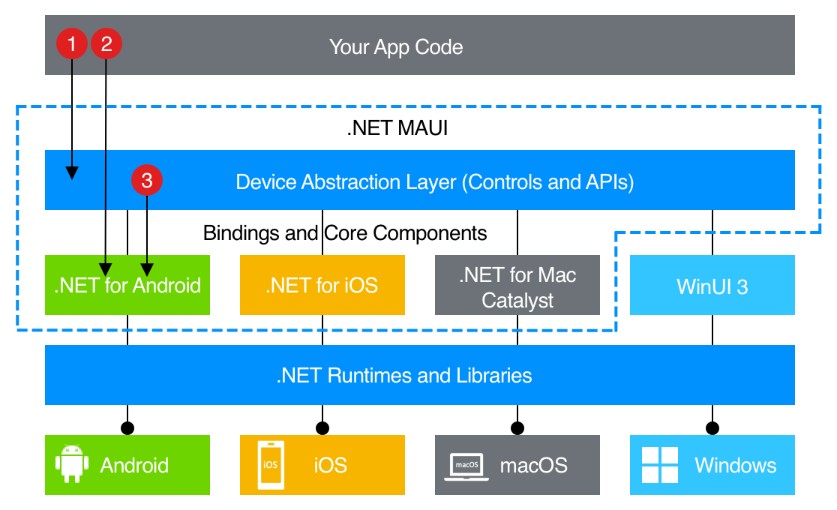
\includegraphics[height=100mm,width=\linewidth,keepaspectratio]{maui-architecture.png}
\vfil

\begin{center}
    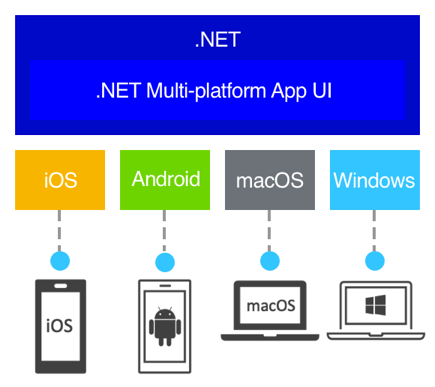
\includegraphics[height=100mm,width=100mm,keepaspectratio]{maui-overview.png}
\end{center}

% page 9
\newpage
\section{Advantages}
\itemize{
    \item CSharp is a robust type safe language so performance oriented projects could be made safely using MAUI.
    \item MAUI has direct access to almost all the native api's using abstractions like File picker, Geolocation, Preferences api,etc.
    \item In Windows, app sizes are extremely small since MAUI uses native components and api's which are inside the Windows SDK, which is installed Windows by default.
    \item Due to the excessive use of native components, MAUI can provide the most performance on heavy tasks which other cross-platform frameworks like flutter or javascript can't.
    \item In Windows and MacOS, apps can be build using ahead of time compilation, which improves app performance and load times even further.
    \item As the MAUI framework is built on top of the .NET library, it has first class support for all the api's available in the .NET library.
    \item No bridging overheads since MAUI has direct access to native api's and UI components.
    \item Fast Build times and initial builds.
    \item MSBuild is faster and more efficient than Gradle, which is used by both Flutter and React Native to build android apps.
    \item Incremental building strategy allows only the changed code to compile and replace existing cached machine code, making the next build really fast.
}

% last page reference links 
\newpage
\section{Reference Links}

\itemize
\item \href{
    https://techexactly.com/blogs/advantages-and-disadvantages-of-using-react-native
}{
    React Native
}
\item \href{
    https://dart.dev/overview
}{
    Dart
}
\item \href{
    https://www.google.co.in/books/edition/NET_MAUI_in_Action/cgDLEAAAQBAJ?hl=en&gbpv=1&dq=.net+maui&pg=PA1&printsec=frontcover
}{
    MAUI
}
\item \href{
    https://www.google.co.in/books/edition/NET_MAUI_in_Action/cgDLEAAAQBAJ?hl=en&gbpv=1&dq=.net+maui&pg=PA1&printsec=frontcover
}{
    MAUI [2]
}
% end of line 
\end{document}